\Level 0 {Introduction}

\TeX's page breaking algorithm is simpler than the line breaking
one. The reason for this is probably that global optimization of
breakpoints, the way it is done in the paragraph algorithm, would take
prohibitively much memory, at least, for the amount of memory that
computers around 1980 had. The algorithm used is related to the `best
fit' algorithm we discussed in the line breaking chapter.

Theoretically, page breaking is a more complicated problem than line
breaking. We will explore the issues in section~\ref{sec:np-page}, but
first we will briefly go into the algorithms that \TeX\ actually uses.

\Level 0 {\TeX's page breaking algorithm}

The problem of page breaking has two components. One is that of
stretching or shrinking available glue (mostly around display math or
section headings) to find typographically desirable breakpoints. The
other is that of placing `floating' material, such as tables and
figures. These are typically placed at the top or the bottom of a
page, on or after the first page where they are referenced. These
`\index{inserts}inserts', as they are called in \TeX, considerably
complicate the page breaking algorithms, as well as the theory.

\Level 1 {Typographical constraints}

There are various typographical guidelines for what a page should look
like, and \TeX\ has mechanisms that can encourage, if not always
enforce, this behaviour.
\begin{enumerate}
\item\label{it:topskip} The first line of every page should be at the
  same distance from the top. This changes if the page starts with a
  section heading which is a larger type size.
\item\label{it:maxdepth} The last line should also be at the same
  distance, this time from the bottom. This is easy to satisfy if all
  pages only contain text, but it becomes harder if there are figures,
  headings, and display math on the page. In that case, a~`ragged
  bottom' can be specified.
\item\label{it:pagenobreak} A page may absolutely not be broken
  between a section heading and the subsequent paragraph or subsection
  heading.
\item\label{it:widowclub} It is desirable that
\begin{enumerate}
\item\label{it:club} the top of the page does not have the last line
  of a paragraph started on the preceding page
\item\label{it:widow} the bottom of the page does not have the first
  line of a paragraph that continues on the next page.
\end{enumerate}
\end{enumerate}

\Level 1 {Mechanisms}

The basic goal of page breaking in \TeX\ is to fill up a box of height
\cs{vsize}. The is the goal size of the material without header and
footer lines. The box is constructed by adding material to the
vertical list until an optimal breakpoint is found. The material
before that breakpoint is then put in \cs{box255}, and the code in
\cs{output}, the `\index{output routine}output routine' is
executed. The command to send a box to the output file is \cs{shipout}.

The typographical rules in the previous section can be realized fairly
simply in \TeX.
\begin{itemize}
\item[\ref{it:topskip}] The vertical location of the first line on a
  page is controlled by \cs{topskip}. If the baseline of the first
  line is closer to the top than this parameter, glue is inserted to
  make up for the difference.
\item[\ref{it:maxdepth}] The vertical location of the last line of a
  page is controlled by \cs{maxdepth}. If the last line of the page is
  deeper than this amount, the reference point of the box is shifted
  down accordingly.
\item[\ref{it:pagenobreak}] Preventing page breaks between vertical
  material of different kinds can be done by the proper use of
  penalties and glue.
\item[\ref{it:club}] A break after the first line
  of a paragraph is prevented by setting the \cs{clubpenalty}.
\item[\ref{it:widow}] A break before the last line
  of a paragraph is prevented by setting the \cs{widowpenalty}.
\end{itemize}

\Level 1 {Breakpoints}

\TeX\ builds up a current page that is a vertical list of material. It
regularly tests whether there is enough material to fill a box of
height \cs{vsize} while incurring a badness less than $10,000$.
The breakpoints are similar to those in the line breaking algorithm,
mostly occurring at a penalty, or at a glue that follows
non-discardable material.

\Level 1 {Some output routines}

The very simplest output routine simply takes the vertical list and
ships it to the output file:
\begin{verbatim}
\output={\shipout\box255}
\end{verbatim}

Slighly more sophisticated, a header and footer are added:
\begin{verbatim}
\output={
  \setbox255=\vbox{ <header>
                    \box255
                    <footer>
                  }
  \shipout\box255
  }
\end{verbatim}

The following example makes the page one line longer if a widow (break
before the last line of a paragraph) occurs. First we save the
original \cs{vsize} and we declare a recognizable value for the
\cs{widowpenalty}:
\begin{verbatim}
\newif\ifEnlargedPage \widowpenalty=147
\newdimen\oldvsize \oldvsize=\vsize
\end{verbatim}
The output routine now works by testing for the widow penalty, and if
it is found, increasing the \cs{vsize} and returning the page material
to the list by \cs{unvbox255}:
\begin{verbatim}
\output={
    \ifEnlargedPage <output the page>
    \else \ifnum \outputpenalty=\widowpenalty
             \global\EnlargedPagetrue
             \global\advance\vsize\baselineskip
             \unvbox255 \penalty\outputpenalty
          \else  \shipout\box255
    \fi   \fi}
\end{verbatim}
Here is the missing bit of code that outputs the enlarged page:
\begin{verbatim}
    \ifEnlargedPage \shipout\box255 
          \global\LargePagefalse
          \global\vsize=\oldvsize
\end{verbatim}

\Level 1 {Insertions}

Floating material, such as tables and figures, are handled by a
mechanism called `insertions'. Insertions fall in different classes,
and insertion material is specified by
\begin{verbatim}
\insert<class number>{ <material> }
\end{verbatim}
If the class number is~$n$, then
\begin{itemize}
\item When the output routine is active, \cs{box}$n$ contains the
  material of insertion class~$n$.
\item \cs{dimen}$n$ specifies the maximum amount of insertion material
  that is allowed to be placed on one page. If there is more material,
  it is split with the remainder carried over to the next page.
\item There are further fine points to this algorithm.
\end{itemize}
Insertions are thus added, for as far as possible, to the page being
formed when the \cs{insert} command is given. \TeX\ has no way of
moving insertions to an earlier page, although moving material to a
later page --~presumable where more space is available~-- is possible.

\Level 0 {Theory of page breaking}
\label{sec:np-page}

At first glance, the page breaking problem is much like the line
breaking problem, except with larger basic blocks, and vertically
instead of horizontally. In the line breaking problem, a long list of
words is broken into lines, adjusting the margins by stretching or
shrinking the interword space. In the page breaking problem, a
vertical list of lines, display formulas, and other vertical material,
is broken into equal sized pages, using the various amounts of
vertical space for taking up the slack.

However, the page breaking problem becomes much harder if we include
the possibility of figures and other floating material. In that case,
the computed badness (the measure we try to minimize in the breaking
process) will include reflect that we want a figure to be close to
pages that reference it, or satisfy other ordering rules involving
references to it. Maybe surprisingly, even rather simple cost
functions make page breaking into an NP-complete problem.

To get an appreciation of the issues, consider this sequence of pages
with figures:

\includegraphics[scale=.8]{pagebreak1}

References to the figures are here indicated with parenthesized
numbers. We see that out of 5~references, 3~are not to a figure on the
same page. However, if we move one line from page~1 to~2, and move
figure~3 forward a page, we get:

\includegraphics[scale=.8]{pagebreak2}

where we see that only one reference is not to the same
page. Unfortunately this is a backward reference.

In the remainder of this chapter we will investigate theoretical
aspects of functions that try to optimize placement of floating
material in a global fashion. It should be noted that this is
considerably more sophisticated than what is implemented in \TeX. The
available algorithm is closer to a `first fit' strategy.

We will investigate two closely related page breaking
algorithms.
We show how a particular form of the page breaking
problem (the `MQ' problem)
is equivalent to the 2-satisfyability problem, which is known
NP-complete. As is usual in the context of proving NP-completeness, we
transform our minimization problem `give the solution with minimum
cost' into a decision problem by asking
`is there a solution with a cost~$\leq B$' where $B$~is some
predetermined bound.

The very similar `ML' problem, which only differs in the form of
the badness function, does have a polynomial time solution.

\Level 1 {The MQ problem is NP-complete}

We consider the MQ page breaking problem: Multiply referenced figures,
and Quadratic badness measure. Under the simplifying assumptions that
each figure takes a whole page, we then have a set
$T=\{t_1,\ldots,t_N\}$ of text blocks and a set $F=\{f_1,\ldots,f_N\}$
of figures and a function $W:T\times F$ such that $W(t_i,f_j)$
describes how many times text block~$i$ references figure~$j$.
We assume a bound $W(t_i,f_j)\leq q(N)$ (where $q$~is a polynomial)
dependent on the size of the problem.

The MQ problem is now the question whether there is an page ordering of
text blocks and figures, that is, a mapping $P:(T\cup F)\rightarrow
\{1,2,\ldots,2N\}$ such that
\[ \begin{array}{cc}P(t_i)<P(t_j)\\ P(f_i)<P(f_j)
    \end{array}\qquad\forall_{1\leq i<j\leq N}
\]
and so that
\[ S=\sum_{i,j}W(t_i,f_j)(P(t_i)-P(f_j))^2\leq B \]

In order to show that this problem is NP-complete, we show that it can
be transformed into an instance of the maximum 2-satisfiability problem. This
means that solving the one problem is equivalent to solving the other,
and since the transformation is done in polynomial time, the two
problems have the same complexity.

The maximum 2-satisfiability (\textsc{max 2-sat} problem can be
formulated as follows. Let there be given $n$~binary
variables~$x_1,\ldots,x_n$ and $m$~clauses~$\{u_1\vee v_1,\ldots,
u_m\vee v_m\}$, where $u_i=x_j$ or $u_i=\neg x_j$ for some~$j$. Given
a bound~$K$, is there a way of setting the $x_i$~variables such that
at least $K$~of the clauses are satisfied? This problem is known to be
NP-complete.

We will now make a pagination problem that `translates' an instance of
the 2-satisfyability problem. That is, given a configuration of binary
variables and clauses and a bound~$K$ to satisfy, we will make a
pagination problem with bound~$B$ such that the one bound is satisfied
if and only if the other is. Then, since \textsc{max 2-sat} is
NP-complete, it follows that this particular pagination problem is
also NP-complete.

\Level 2 {Construction of the translation}

We make the translation between the two types of problems by
constructing the page assignment function~$P$, and the weight
function~$W$. There are three aspects we need to take care of, so we
let $B=B_1+B_2+B_3$, and we will determine the $B_i$~bounds
separately.

First of all we set $W(t_i,f_i)=b_1$ sufficiently large that only
configuration with $|P(t_i)-P(f_i)|=1$ will satisfy the bound. (Recall
that the badness is a sum of $W(t_i,f_j)(P(t_i)-P(f_j))^2$ terms.)
To allow for the pages to be ordered this way, we
let~$B_1=Nb_1$. The $b_1$ quantity will be defined in terms of
$B_2$ and~$B_3$ as
\[ b_1 = \lceil (B_2+B_3)/3\rceil+1 \]
Supposing that at least one $t_i,f_i$ pair is not adjacent, then it
follows from this bound that the badness will be
\[ S\geq (N-1)b_1+2^2b_1=(N+3)b_1>B \]
where the $N-1$ corresponds to the pairs that are adjacent, and the
$2^2$~to at least one pair at distance~2.

Since
text blocks and are next to each other, the only remaining question is
which comes first. This limits the number of cases we need to consider
in the remainder of this proof.

Now let parameters $n$~for the number of variables and~$m$ for the
number of clauses be as described above, then our pagination problem
will have $N$~text blocks and figures, where~$N=2n+2m$.  The first
$4n$ pages encode the values of the variables~$x_i$, with each
consecutive 4~pages corresponding to one variable:
\[ \begin{array}{lllll}
4i-3&4i-2&4i-1&4i\\
t_{2i-1}&f_{2i-1}&f_{2i}&t_{2i}&\quad\hbox{if $x_i$ is true}\\
f_{2i-1}&t_{2i-1}&t_{2i}&f_{2i}&\quad\hbox{if $x_i$ is false}
\end{array}
\]
To ensure that these are the only configuration that will satisfy the
bound, set $W(t_{2i-1},f_{2i})=W(f_{2i-1},t_{2i})=b_2$ large enough.
Either of the above patterns then contributes $2\cdot 2^2b_2=8b_2$, while
the other possibilities ($t\,f\,t\,f$ and $f\,t\,f\,t$) would
contribute $(1^2+3^2)b_2=10b_2$.

Correspondingly, we allow a bound of $B_2=4b_2\sum(i-j)^2$ where
$i,j$~range over the pairs that satisfy $W(t_i,f_j)=b_2$.  Defining 
\[ b_2=8(m-k)+5 \]
is sufficient to make violation of this condition
outweigh the gain from more clauses being satisfied.

Next, the $4m$ remaining pages will encode the clauses in a similar
manner:
\[ \begin{array}{lllll}
4n+4j-3&4n+4j-2&4n+4j-1&4n+4j\\
t_{2n+2j-1}&f_{2n+2j-1}&&&\quad\hbox{if $u_j$ is true}\\
f_{2n+2j-1}&t_{2n+2j-1}&&&\quad\hbox{if $u_j$ is false}\\
&&t_{2n+2j}&f_{2n+2j}&\quad\hbox{if $v_j$ is true}\\
&&f_{2n+2j}&t_{2n+2j}&\quad\hbox{if $v_j$ is false}
\end{array}
\]
Further conditions on~$W$ ensure that the $u_j$~variables indeed
correspond to the proper~$x_i$. For instance
\[ W(t_{2n+2j-1},f_{2i}) = W(t_{2i}=f_{2n+2j-1})=b_2
    \quad\hbox{if $u_j=x_i$}
\]
This term contributes $2d^2b_2$ to the badness, where $d$~is twice the
difference between the subscripts, in this case $d=(2n+2j-2i)$.
With a mismatch, a $t$~and~$f$ page assignment are reversed, so the
contribution becomes $\bigl((d-1)^2+(d+1)^2\bigr)=2(d^2+1)b_2$.

Proper truth values of the clauses are enforced as follows. Observe
that the
combination where $u_j$~and~$v_j$ are both false is the only one that
gives a false result. This corresponds to the pagination
\[ \begin{array}{llll}f_{2n+2j-1}&t_{2n+2j-1}&f_{2n+2j}&t_{2n+2j}
    \end{array}
\]
In this configuration $f_{2n+2j_1}$ and~$t_{2n+2j}$ are spread the
furthest apart, so we penalize that with
\[ W(t_{2n+2j},f_{2n+2j_1})=5, \qquad
   W(t_{2n+2j-1},f_{2n+2j})=3.
\]
This gives a contribution of~32 for the three true cases, and 48~for
the false result. Correspondingly,
to allow for $K$ clauses to be satisfied we allow $B_3=48(m-K)+32K$.

Finally, by defining the polynomial $q(i)=64(i+1)^4$, we have
$q(N)>b_1\geq b_2>5>3$, so $W$~is bounded as required.

\Level 2 {NP-completeness}

In order to establish NP-completeness of the problem~\textsc{MQ}, we need to
establish that something is a true instance of \textsc{Max 2-sat} iff
the translated instance is true for~\textsc{MQ}.

Given
a truth assignment of the~$x_i$s that makes $K$~clauses true,
we can now construct
a pagination~$P$ with a satisfied bound of~$B$.

Conversely, let a pagination with bound~$B$ be given, then the
corresponding truth assignment makes $K$~clauses true. To see this,
inspect each of the details of the translation between the problems,
and observe that any violation will cause the bound~$B$ to be exceeded.

\Level 1 {The ML problem has a polynomial time solution}

The `ML' problem (Multiply referenced figures, Linear badness
function) is identical to MQ, except for the form of the badness function.
Having a linear badness function makes it
possible to solve this problem by dynamic programming in linear time.

As in MQ, we have text blocks~$t_i$ and figures~$f_j$ that take up
whole pages.
We generalize the problem slightly to having different numbers of text
and figure blocks:
\[ T=\{t_1,\ldots,t_N\},\qquad F=\{f_1,\ldots,f_M\} \]
The function $W:T\times F$ is such that $W(t_i,f_j)\geq\nobreak 0$
describes how many times text block~$i$ references figure~$j$.

The ML problem is now the question whether, given the above, and given
a bound~$B$, there is an page ordering of
text blocks and figures, that is, a mapping $P:(T\cup F)\rightarrow
\{1,2,\ldots,M+N\}$ such that
\[ \begin{array}{cc}P(t_i)<P(t_j)\\ P(f_i)<P(f_j)
    \end{array}\qquad\forall_{1\leq i\leq N,1\leq j\leq M}
\]
and so that
\newcommand\WPP[2]{\WPPf{#1}{#2}{#1}{#2}}
\newcommand\WPPf[4]{W(t_#1,f_#2)\left|P(t_#3)-P(f_#4)\right|}
\[ S=\sum_{i,j}\WPP ij \leq B \]

\Level 2 {Dynamic programming solution}

The key to a dynamic programming solution of ML is to identify
subproblems. The subproblem we consider is
\begin{quote}
Given $i$ text blocks and $j$ figures, what is the least badness of
placing these on the first $i+j$ pages. Call this partial badness $B_{ij}$. 
\end{quote}
The problem
here is the `dangling' references $(t_r,f_s)$ with $r>i,s\leq j$ or
$r\leq i,s>j$. The measure $R_{i,j}$ is defined as the
number of dangling references after these blocks and figures
have been placed.

A~dangling reference is either
\begin{description}
\item[A forward reference:] A text block refering to a figure not yet
  placed. The number of forward references from the $i+j$ block is
\[ F_{ij}=\sum_{{1\leq r\leq i\atop j<s\leq M}} W(t_r,f_s) \]
\item[A backward reference:] A figure that will be reference on a text
  block not yet placed.) The number of backward references from
  the $i+j$ block is
\[ B_{ij} = \sum_{{i< r\leq N\atop 1\leq s\leq j}} W(t_r,f_s) \]
\end{description}
which makes $R_{ij}=F_{ij}+B_{ij}$.

\begin{figure}[ht]
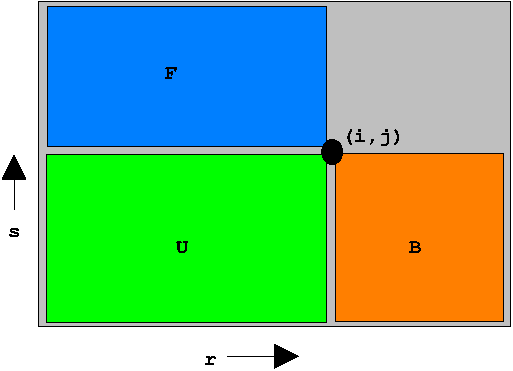
\includegraphics{linear-bad}
\caption{The $F_{ij}$, $B_{ij}$, and $U_{ij}$ areas in $(r,s)$ space}
\label{fig:FBU}
\end{figure}

For badness calculations involving dangling references,
we count only the part to the boundary of
the $i,j$ region. Formally:
\[ B_{ij} = B^{(1)}_{ij}+B^{(2)}_{ij} \]
where
\[ B^{(1)}_{ij} =
     \sum_{{r\leq i\atop s\leq j}}\WPP rs
\]
is the part of the badness due to references that are fully resolved
within the pages already placed; the part of the badness due to
dangling references is
\begin{figure}[ht]
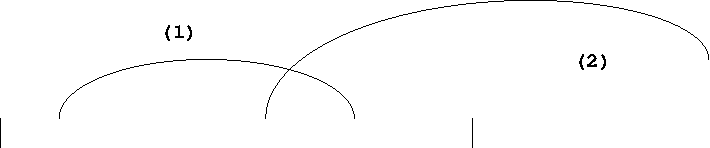
\includegraphics[scale=.7]{dangle1}
\caption{Resolved and dangling references of a block of pages}
\label{fig:dangle1}
\end{figure}
\newcommand\ElRS{\mathop\ell(i,j;r,s)}
\[ B^{(2)}_{ij} =
     \sum_{{r>i\atop s\leq j}} W(t_r,f_s)\ElRS
   + \sum_{{r\leq i\atop s> j}} W(t_r,f_s)\ElRS
\]
where
\[ \ElRS = \cases{i+j-P(f_s)&if $r>i$\cr i+j-P(t_r)&if $s>j$}
\]
describes the part of the arc between $t_r$ and~$f_2$ that lies in the
first $i+j$ pages. These two types of arcs are illustrated in
figure~\ref{fig:dangle1}.

Figure~\ref{fig:dangle2} illustrates how reference arcs change status
when we go from $i+j-1$ to $i+j$ pages, say by placing text
block~$t_i$:
\begin{figure}[ht]
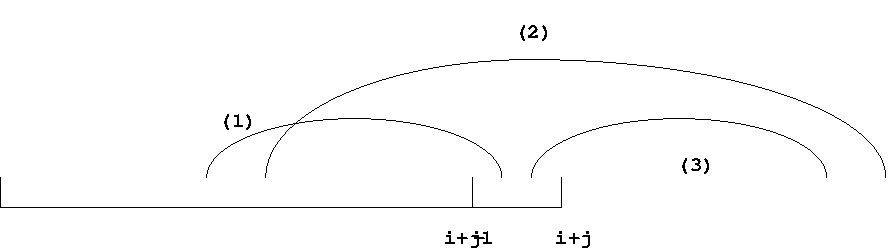
\includegraphics[scale=.6]{dangle2}
\caption{Change in status of resolved and dangling references
upon extending a block of pages}
\label{fig:dangle2}
\end{figure}
\begin{enumerate}
\item[(1)] References that were unresolved with references originating
  in~$t_i$ move their contribution from the $B^{(2)}$ term to the
  $B^{(1)}$ term. (Note that a reference to a page one location
  outside the current block is already fully counted in the badness.)
\item[(2)] Dangling references that stay unresolved increase their
  contribution to the $B^{(2)}$ term by $(\sum_{r\leq i-1,s>j} +
  \sum_{r>i-1,s\leq j}) W(t_r,f_s)$
\item[(3)] Arcs that used to fall completely outside the page block,
  but that are now dangling in the new page block, add a contribution
  of $\sum_{r=i,s>j}W(t_r,f_s)$ to the $B^{(2)}$ term.
\end{enumerate}
$\sum_{r>i,s\leq j}W(t_r,f_s)$
In sum, $B_{ij}=B_{i-1,j}+R_{ij}$. The same story holds for extending
$i+j-1$ pages by placing figure~$f_j$, so we have the recurrence
\[ B_{ij} = \min(B_{i-1,j},B_{i,j-1})+R_{ij}. \]

We still need to compute the $R_{ij}$ quantities, describing the
number of dangling references from placing $i$~text blocks and
$j$~figures.
Above we saw  $R_{ij}=F_{ij}+B_{ij}$.
For efficient calculation of these sums, it is convenient to make a
table of
\[ U_{ij} = \sum_{{1\leq r\leq i\atop 1\leq s\leq j}}W(t_r,f_s) \]
which takes time~$O(NM)$, that is, quadratic in the total number of
pages. Then 
\[ R_{ij} = U_{iM}+U_{Nj}-2U_{ij}, \]
as is easily seen from figure~\ref{fig:FBU}.

\Level 1 {Discussion}

It is interesting to note that
certain details of the NP-completeness proof of MQ
rely on the quadratic badness
function, rather than on more `structural' properties of the problem.
\begin{594exercise}
Find a place in the NP-completeness proof of MQ that uses the
quadratic badness function, and show that the underlying fact does not
hold for linear functions. Does it hold for other functions than
quadratic?
\end{594exercise}
\begin{answer}
In enforcing the same values for the $x_i$ and $u_j$ values, the proof
used that 
\[ (d+1)^+(d-1)^2>2d^2. \]
The general requirement for the badness function is
\[ f(n+1)+f(n-1)>2f(n), \]
which is satisfied for polynomial badness functions that increase
faster than linear. The statement is that $f(n)$ is less than the
average of the surrounding values, so in fact any convex function
would work.
\end{answer}

Similarly, ML only has a dynamic programming solution thanks to the
linear badness function.
\begin{594exercise}
Explain how the linearity of the badness function is essential for the
dynamic programming solution of ML.
\end{594exercise}
\begin{answer}
Linearity is used in constructing partial badness, counting only the
part of the reference arc to the boundary of the $(i,j)$ block.
That would not work for non-linear badness functions.

You can see the same use of linearity in the fact that badness gets
updated by $W(t_i,f_j)$ when a new block is placed.  This
means that each unit distance contributes the same amount, in other
words that the badness is linear in the distance.
\end{answer}

\begin{594exercise}
The discussion of the ML problem only gave the cost computation. How
can the actual page assignment be derived from the given construction?
What is the time and space complexity of this part of the algorithm?
\end{594exercise}
\begin{answer}
Look at the relation
\[ B_{ij} = \min(B_{i-1,j},B_{i,j-1})+R_{ij}. \]
Starting at $i=N$, $j=M$, find for each $ij$ point the minimum of
$B_{i-1,j}$ and~$B_{i,j-1}$; that must have been the previous step.
\end{answer}
